\documentclass[11pt]{article}
\usepackage[a4paper,margin=2.4cm]{geometry}
\usepackage{amsmath,amssymb}
\usepackage{booktabs}
\usepackage{array}
\usepackage{xcolor}
\usepackage{listings}
\usepackage{titlesec}
\usepackage{enumitem}
\usepackage{hyperref}
\usepackage{caption}
\usepackage{subcaption}
\usepackage{graphicx}
\usepackage{colortbl}

\definecolor{headerblue}{RGB}{47,79,111}
\definecolor{codegray}{RGB}{242,242,242}
\definecolor{warnred}{RGB}{245,230,230}

\titleformat{\section}{\normalfont\Large\bfseries\color{headerblue}}{\thesection}{1em}{}
\titleformat{\subsection}{\normalfont\large\bfseries\color{headerblue}}{\thesubsection}{1em}{}

\lstset{
  backgroundcolor=\color{codegray}, basicstyle=\ttfamily\small, frame=single,
  rulecolor=\color{gray!40}, breaklines=true, columns=fullflexible, keepspaces=true,
  xleftmargin=4pt, xrightmargin=4pt, aboveskip=8pt, belowskip=10pt,
}

\hypersetup{colorlinks=true, linkcolor=headerblue, urlcolor=headerblue, citecolor=headerblue}
\emergencystretch=3em
\sloppy

\title{\textbf{Randers-UMAP on the Swiss Roll:}\\[2pt]
\textbf{Three Initialisation Strategies and the Ramp Mechanism}\\[4pt]
\Large\color{headerblue}Progress Report, Week of August 7--12}
\author{Rümeysa Bilik \\ \textit{Max Planck Institute for Mathematics in the Sciences} \\ \textit{Supervised by Prof. Jürgen Jost}}
\date{August 12, 2026}

\begin{document}
\maketitle

\section{Methodology recap}
\label{sec:methodology}

All three pipelines below share the same skeleton, so this section is intentionally short.

\textbf{Distance matrix.} \texttt{randers\_bridge.py::compute\_dist\_matrix} turns $(X,\omega)$
into an asymmetric geodesic distance matrix $D_{\mathrm{asym}}$: build a neighbourhood graph on
$X$, perturb each edge weight by $\langle\omega_i,\,x_j-x_i\rangle$, run directed shortest-path.
This week the neighbourhood-graph step was rewritten (\S\ref{sec:progress}) to match
\href{https://github.com/lwileczek/isomap}{lwileczek/isomap}'s threshold construction instead of
scikit-learn's $k$-NN graph.

\textbf{Randers metric.} Every method ultimately positions each node $i$ at $y_i\in\mathbb R^2$
together with a drift vector $b_i$, $\lVert b_i\rVert\le1-\delta$, so that
\begin{equation}
F(i\to j) \;=\; \lVert y_j-y_i\rVert \;+\; \langle b_i,\,\hat e_{ij}\rangle
\label{eq:randers}
\end{equation}
approximates $D_{\mathrm{asym}}[i,j]$. The three pipelines differ only in \emph{how $Y$ and $B$ are
initialised} and \emph{what update rule} then refines $Y$ -- see \S\ref{sec:three-methods}.

\textbf{Force-directed update (used by two of the three).}
\texttt{randers\_umap.py::randers\_umap\_fit} lays $Y$ out with a dense, full-batch UMAP-style
attraction/repulsion graph layout, not gradient descent against a loss. $D_{\mathrm{asym}}$ is
first turned into a fuzzy membership graph $\mu_{ij}\in[0,1]$ exactly as in UMAP itself (Section
3.1 of the original paper): a per-point $\rho_i,\sigma_i$ calibration on the $k$ nearest neighbours
so every node's total soft-neighbourhood weight matches $\log_2 k$. The drift then enters the
layout by replacing the ordinary embedding distance and force direction with
\begin{equation}
\rho_{i\to j} = \lVert y_j-y_i\rVert + b_i\cdot(y_j-y_i), \qquad
g_{ij} = \hat e_{ij} + b_i,
\label{eq:rho-g}
\end{equation}
inside UMAP's own attractive/repulsive coefficients $\mathrm{attr}(\rho),\mathrm{rep}(\rho)$ (the
usual $(a,b)$ curve fit to \texttt{min\_dist}/\texttt{spread}). The net force on node $i$ is
\begin{equation}
\mathrm{force}_i \;=\; \sum_j \Big[\mu_{ij}\,\mathrm{attr}(\rho_{ij}) \;-\; (1-\mu_{ij})\,\mathrm{rep}(\rho_{ij})\Big]\, g_{ij},
\end{equation}
and $Y$ is updated by pure force accumulation, $Y\leftarrow Y+\eta\,\mathrm{force}$, every epoch.
Setting $b_i\equiv0$ everywhere recovers vanilla UMAP exactly, since then $\rho=\lVert
y_j-y_i\rVert$ and $g=\hat e_{ij}$.

\textbf{Locating the drift via virtual points.} $B$ itself is not learned by this force loop --
\texttt{B\_fixed} is computed once, \emph{before} training, and never updated afterwards (only its
\emph{magnitude} is phased in, see the ramp mechanism, \S\ref{sec:ramp}). The main construction
(Isomap and SVD-RADAR pipelines, \S\ref{sec:three-methods}) locates it geometrically: for every
real point $x_i$, place an imaginary target
\begin{equation}
x_i^{\mathrm{virt}} := x_i + \omega_i
\end{equation}
in the same ambient space -- a genuine position, not an abstract offset, since $\omega$ is
represented in the same coordinates as $X$. All $2n$ real+virtual points are then embedded
\emph{jointly} with plain, drift-off UMAP ($b\equiv0$ in Eq.~\eqref{eq:rho-g}) on their symmetric
geodesic distance. The located drift is simply the displacement between the two embedded images of
the same node,
\begin{equation}
B_{\mathrm{located}} \;:=\; y_i^{\mathrm{virt}} - y_i^{\mathrm{real}}, \qquad
b_i \leftarrow b_i\cdot\min\!\Big(1,\ \tfrac{1-\delta}{\lVert b_i\rVert}\Big),
\label{eq:located}
\end{equation}
clipped to the Randers bound. $B_{\mathrm{located}}$ is then frozen and passed as
\texttt{B\_fixed} to the real (asymmetric) embedding: it still shapes $Y$'s force every epoch
through Eq.~\eqref{eq:rho-g}, but its own value never changes for the rest of training -- it is
rigidly ``attached'' to node $i$ and rides along as $y_i$ moves.

\section{The ramp mechanism}
\label{sec:ramp}

\subsection{What it is}

\texttt{randers\_umap\_fit} accepts a frozen drift field \texttt{B\_fixed} (computed once,
attached to each node, never retrained -- see \S\ref{sec:three-methods}). A scalar schedule $s(\tau)$
optionally controls how much of that frozen field is actually applied at epoch $\tau$:
\begin{equation}
s(\tau) = \begin{cases} 0 & \tau/T \le 0.30 \\ (\tau/T-0.30)/0.40 & 0.30<\tau/T<0.70 \\ 1 & \tau/T\ge0.70\end{cases},
\qquad B(\tau) = s(\tau)\cdot B_{\mathrm{fixed}},
\label{eq:ramp}
\end{equation}
$T$ the total epoch count. \texttt{ramp=False} fixes $s\equiv1$: the frozen field is applied at
full strength from epoch 0. Only $s$ changes with $\tau$ -- $B_{\mathrm{fixed}}$'s direction is
never touched, so this is not a re-optimisation of $B$, only a magnitude schedule.

\subsection{Why full strength from epoch 0 can fail}

From \eqref{eq:randers}, Cauchy--Schwarz bounds the drift term:
\begin{equation}
\big|\,b_i\cdot(y_j-y_i)\,\big| \;\le\; \lVert b_i\rVert\cdot\lVert y_j-y_i\rVert.
\end{equation}
So $\rho_{i\to j}\in\big[(1-\lVert b_i\rVert)d_{ij},\ (1+\lVert b_i\rVert)d_{ij}\big]$. For a
well-behaved node ($\lVert b_i\rVert\approx0.05$, the typical case at $n=300$, see
Table~\ref{tab:clip}) this is a gentle $\pm5\%$ perturbation of distance. For a node sitting at the
Randers clip boundary ($\lVert b_i\rVert\approx0.99$) it is a $\pm99\%$ swing: $\rho$ can fall to
$\approx0.01\,d_{ij}$ or rise to $\approx1.99\,d_{ij}$ for the \emph{same} pair of points, depending
only on which node is source. The $(a,b)$ attraction/repulsion curve was calibrated
(\texttt{min\_dist=0.1}, \texttt{spread=1.0}) assuming $\rho$ behaves like an ordinary,
well-scaled UMAP distance -- not one that can swing this violently. Applying that swing at full
strength ($s=1$) from epoch~0, while $Y$ is still the compact, just-finished output of the locate
step and has not yet found its natural scale, produces erratic per-edge forces for every saturated
node: a minority of nodes get flung to extreme positions while the majority, left with only
ordinary (and, at this $n$, comparatively weak dense-repulsion) attraction, collapse toward a
shared centroid.

\subsection{Empirical evidence, $n=2000$}
\label{sec:ramp-data}

\begin{table}[h]
\centering
\begin{tabular}{@{}lrrrr@{}}
\toprule
run & locate epochs & mean $\lVert b\rVert$ & max $\lVert b\rVert$ & clipped (of 2000) \\
\midrule
$k=20$, default locate (500 ep.) & 500 & 0.053 & 0.990 & 11 \\
$k=12$, short locate (100 ep.) & 100 & 0.143 & 0.990 & 206 \\
\bottomrule
\end{tabular}
\caption{Locate-step convergence, not $k$, is the dominant driver of $B_{\mathrm{located}}$'s
saturation -- see the caveat in \S\ref{sec:progress}.}
\label{tab:clip}
\end{table}

With \texttt{ramp=False} on the 206/2000-saturated run: apply-step epoch~0 already shows
mean~$|\rho-d|=0.797$ (against $0.124$ at $n=300$, 0 saturated nodes), and the final embedding
extent reaches $149.6$ (against $19$--$24$ at $n=300$) -- see Figure~\ref{fig:ramp-off}: a tight
central clump with a handful of nodes flung to the edges. Switching only \texttt{ramp=True}, same
data, same seed, same $B_{\mathrm{located}}$: Figure~\ref{fig:ramp-on} shows a clearly organised,
colour-separated layout by epoch~20--40, because $s\approx0$ during the first $30\%$ of epochs lets
$Y$ spread under ordinary UMAP forces \emph{before} the saturated nodes' extreme drift is switched
on.

\begin{figure}[h]
\centering
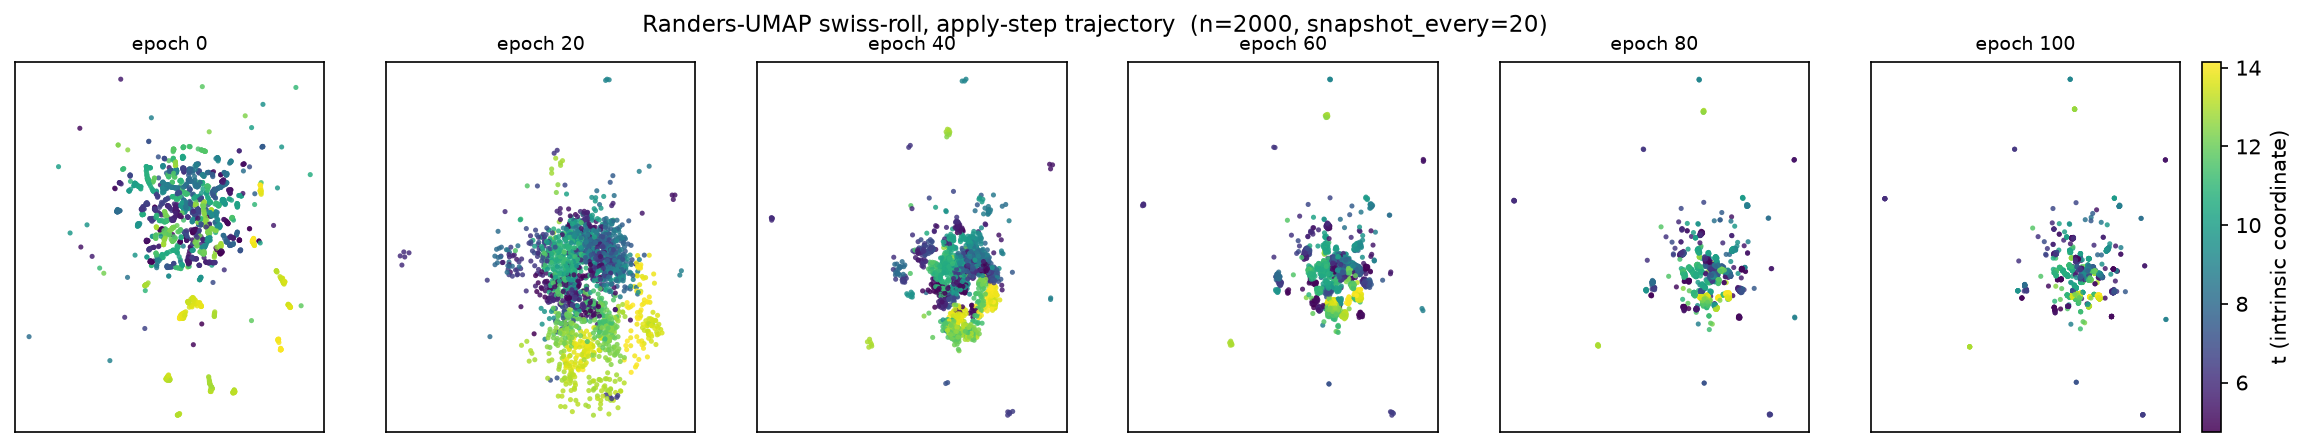
\includegraphics[width=\linewidth]{report_figs/ramp_off_collapse.png}
\caption{\texttt{ramp=False}, $n=2000$: central collapse plus flung-out outliers.}
\label{fig:ramp-off}
\end{figure}

\begin{figure}[h]
\centering
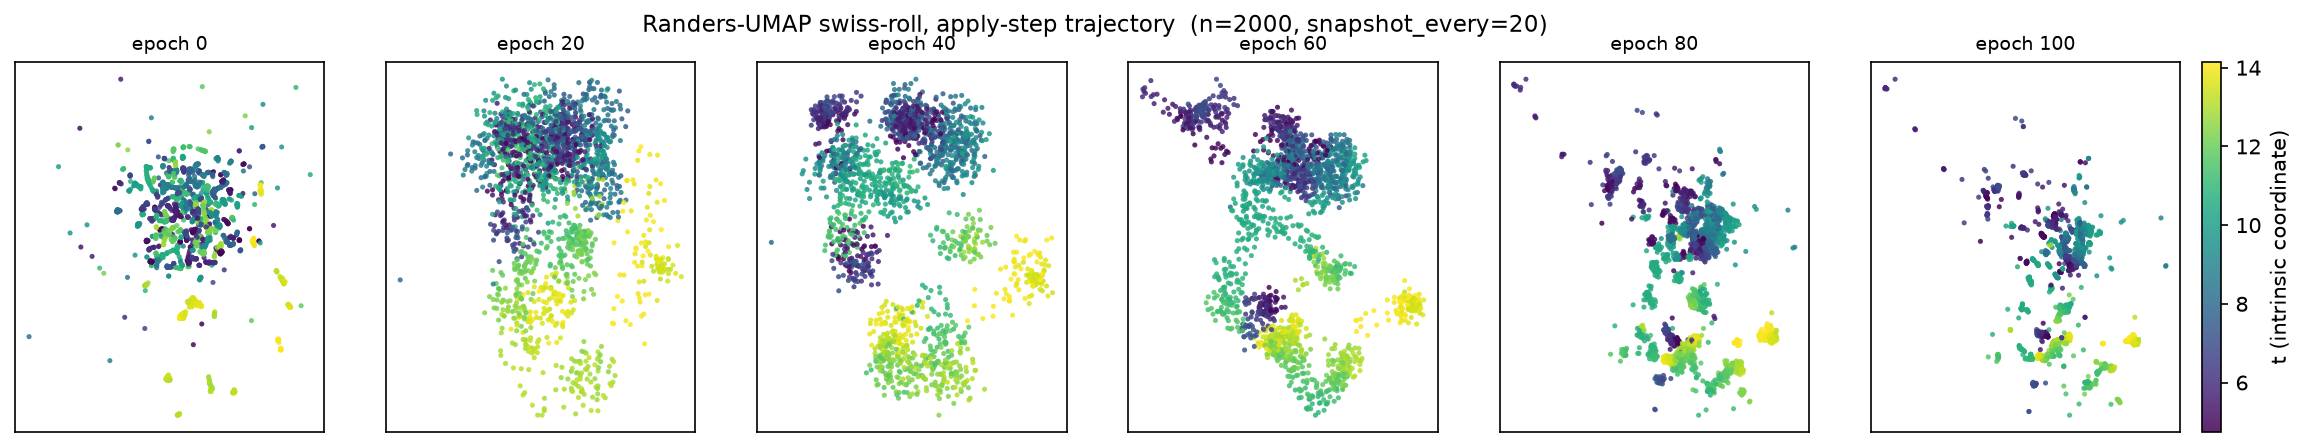
\includegraphics[width=\linewidth]{report_figs/ramp_on_organized.png}
\caption{\texttt{ramp=True}, identical run otherwise: organised, colour-separated layout.}
\label{fig:ramp-on}
\end{figure}

\subsection{Caveat -- not yet fully isolated}
Table~\ref{tab:clip}'s two runs differ in \emph{both} $k$ (20 vs.\ 12) \emph{and} locate-step
epoch count (500 vs.\ 100) simultaneously, because the short-locate-epoch run was originally set up
for fast iteration, not as a controlled comparison. The saturation jump is more plausibly explained
by the shorter, under-converged locate step than by $k$ itself (see \S\ref{sec:progress}'s $k$
discussion, which is a separate, independently-verified finding). A clean single-variable rerun
($k=12$, locate-epochs=500) is on the list below (\S\ref{sec:next}) but has not been run yet.
\texttt{ramp=True} was adopted regardless because it makes the pipeline robust to a saturated
$B_{\mathrm{located}}$ \emph{whatever} its source, which is a reasonable thing to want independent
of this open question. \texttt{ramp} is now a CLI flag (\texttt{--ramp}, default off) on all three
scripts in \S\ref{sec:three-methods}, so it can be toggled without editing code.

\section{Three initialisation strategies}
\label{sec:three-methods}

All three now share the same force-directed update mechanism, Eq.~\eqref{eq:rho-g}. They differ
only in how $(Y_{\mathrm{init}}, B)$ is obtained.

\subsection{Isomap -- \texttt{run\_swiss\_roll.py}}
$D_{\mathrm{asym}}$ from \texttt{compute\_dist\_matrix} (the Isomap-style geodesic backbone). $B$
and $Y_{\mathrm{init}}$ both come directly from the virtual-point locate step described in
\S\ref{sec:methodology} (Eq.~\eqref{eq:located}): $B:=B_{\mathrm{located}}$, and
$Y_{\mathrm{init}}:=y^{\mathrm{real}}$ from that same joint embedding. No separate initialisation
step beyond the locate step itself. Figure~\ref{fig:three-methods}(a).

\subsection{isumap -- \texttt{run\_swiss\_roll\_isumap.py}}
$D_{\mathrm{asym}}$ comes from \texttt{distance\_graph\_generation.py} -- isumap's own, untouched
library code (local $\rho_i/\sigma_i$ normalisation, star-graph restriction, fuzzy $t$-conorm
merge -- see the file-by-file walkthrough discussed separately). This method has no notion of
$\omega$ at all -- its asymmetry comes purely from the directed $k$-NN structure isumap itself
builds -- so there is no virtual target to locate. $B$ instead comes from a one-shot SVD of the
skew-symmetric part, $B:=\mathrm{svd\_init}(D_{\mathrm{asym}}^\top-D_{\mathrm{asym}})[:, :d]$,
clipped to the Randers bound. $Y_{\mathrm{init}}$ is whatever \texttt{randers\_umap\_fit}'s own
spectral initialisation gives on $D_{\mathrm{asym}}$ (no separate locate step here either).
Figure~\ref{fig:three-methods}(b).

\subsection{SVD-RADAR -- \texttt{run\_swiss\_roll\_svd\_radar.py}}
Same $D_{\mathrm{asym}}$ as the Isomap pipeline (true $\omega$). $B$ is \emph{still} the located
construction above -- unchanged, because $B$ needs the true $\omega$ field to locate against, and
SVD-of-Delta is a structurally different signal not yet validated as a substitute. The only thing
that changes relative to \S3.1 is $Y_{\mathrm{init}}$: instead of the locate step's own
$y^{\mathrm{real}}$, $Y_{\mathrm{init}}:=\mathrm{svd\_init}(D_{\mathrm{asym}})[:,:d]$ (RADAR-style
truncated SVD of the asymmetric matrix itself, no double-centering). This isolates a single
variable against \S3.1: does an SVD-derived starting position help or hurt, everything else held
fixed? Figure~\ref{fig:three-methods}(c). (This script previously used a completely different
mechanism -- SVD init feeding an Adam/Finsler-loss regression, \texttt{finsler\_mds\_freeB} -- see
\S\ref{sec:progress}.)

\begin{figure}[h]
\centering
\begin{subfigure}{0.32\textwidth}
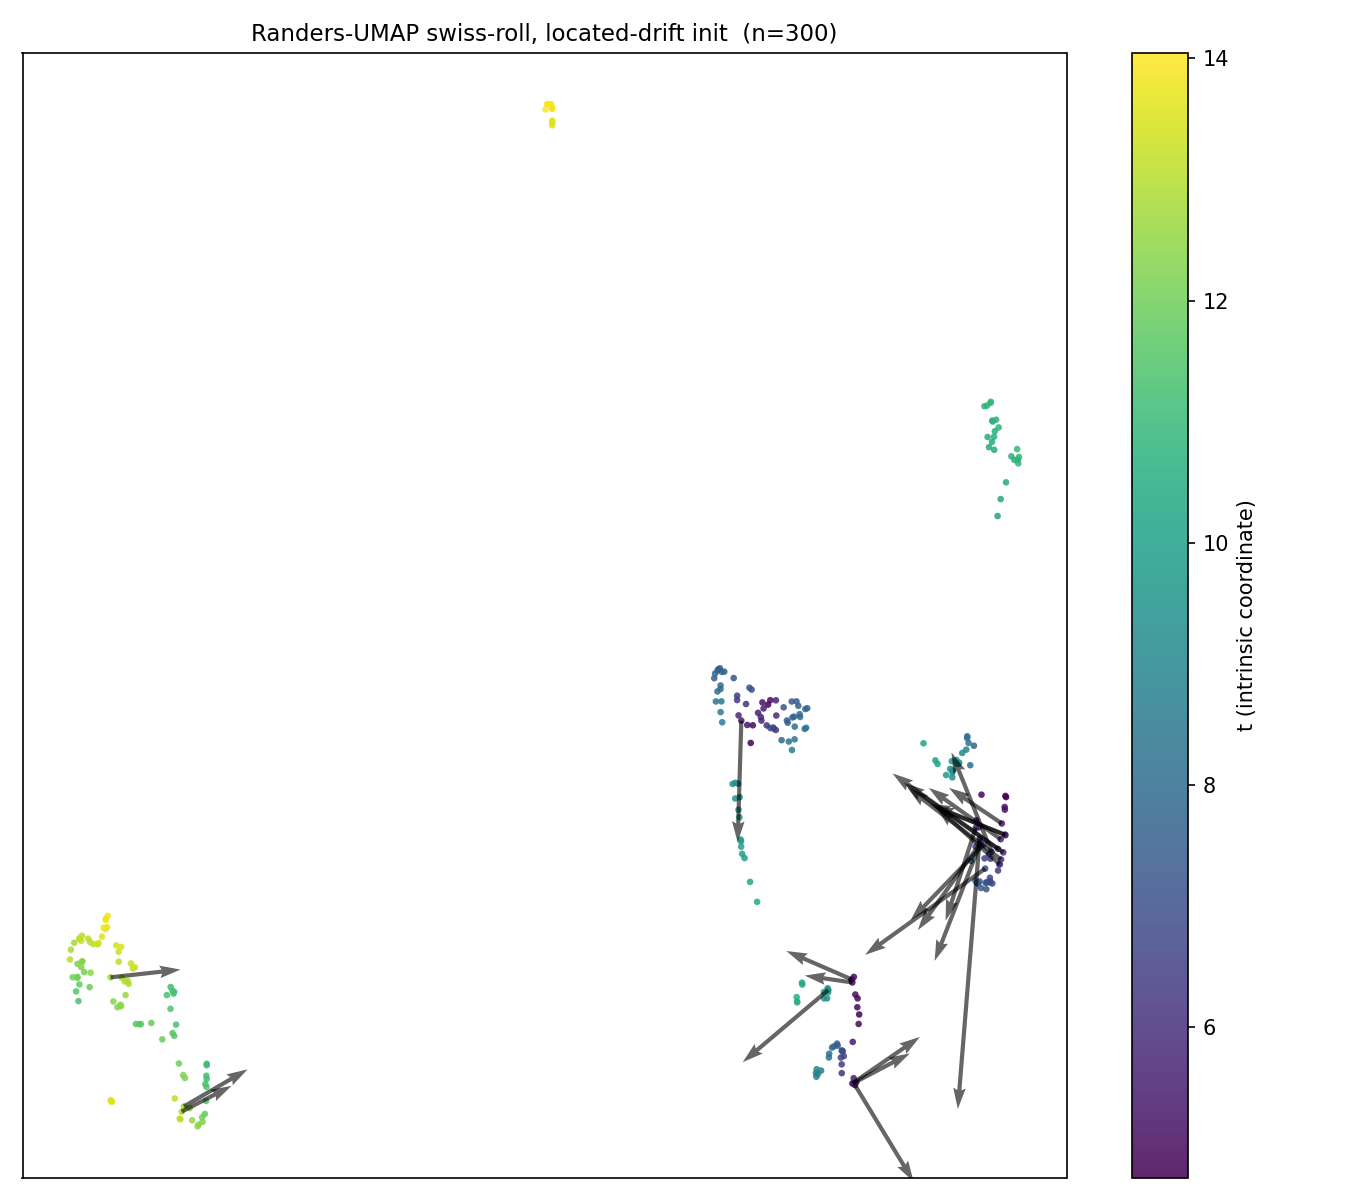
\includegraphics[width=\linewidth]{report_figs/final_isomap.png}
\caption{Isomap (located $Y,B$)}
\end{subfigure}
\begin{subfigure}{0.32\textwidth}
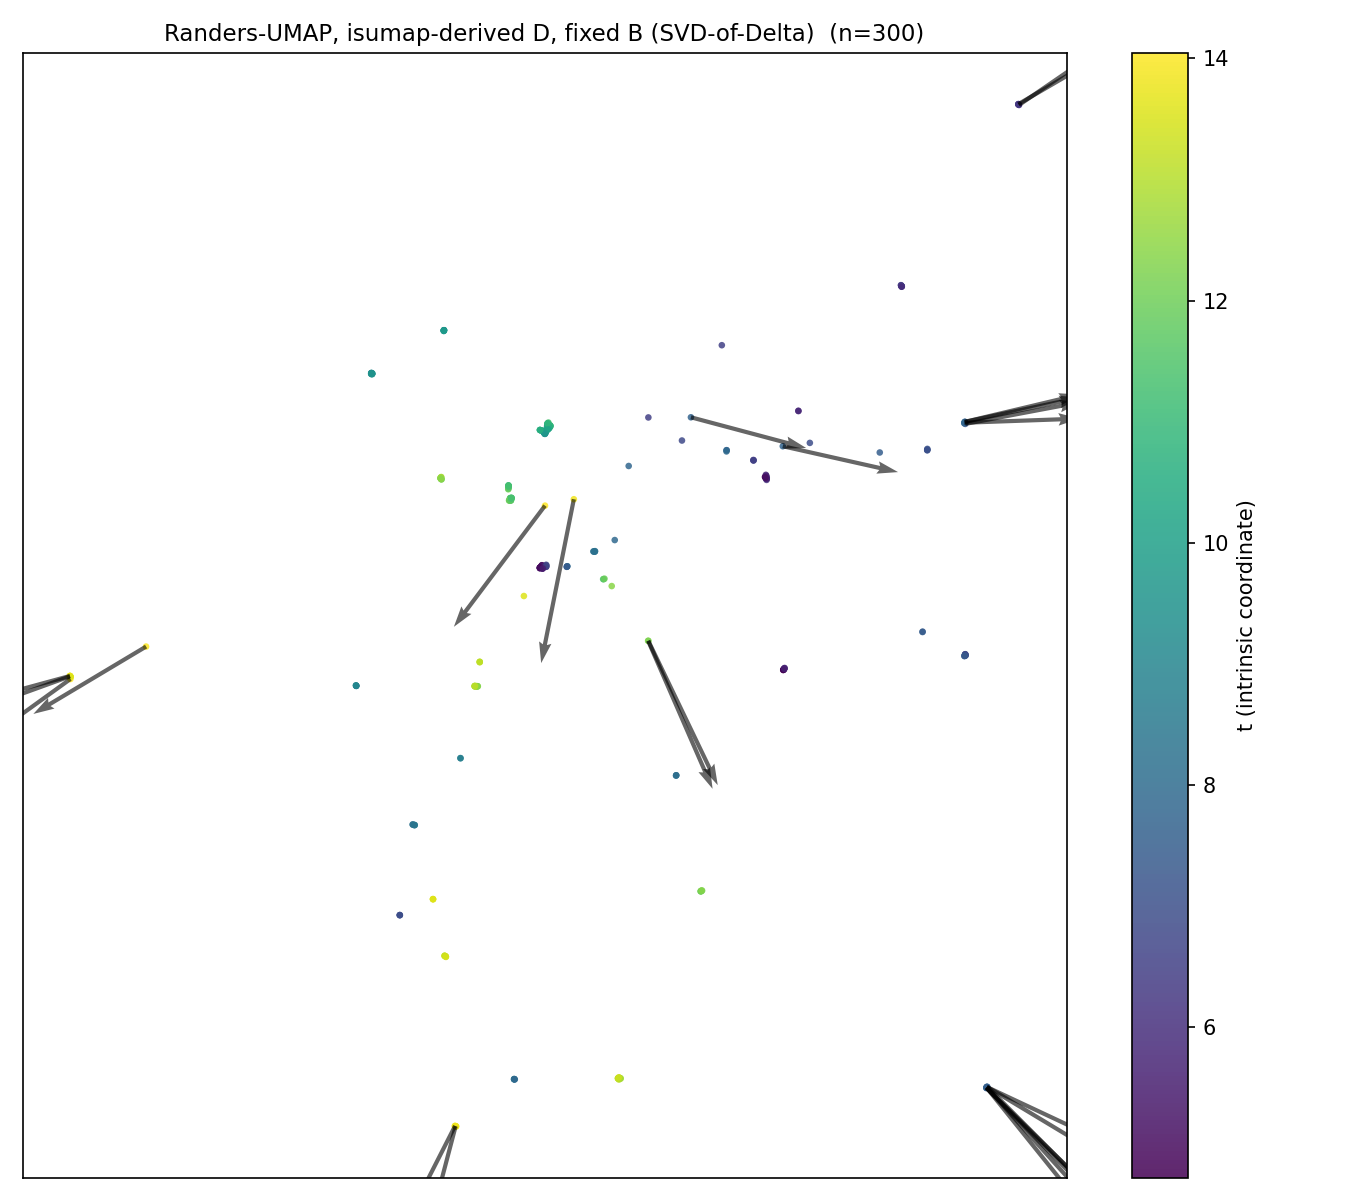
\includegraphics[width=\linewidth]{report_figs/final_isumap.png}
\caption{isumap (SVD-of-Delta $B$)}
\end{subfigure}
\begin{subfigure}{0.32\textwidth}
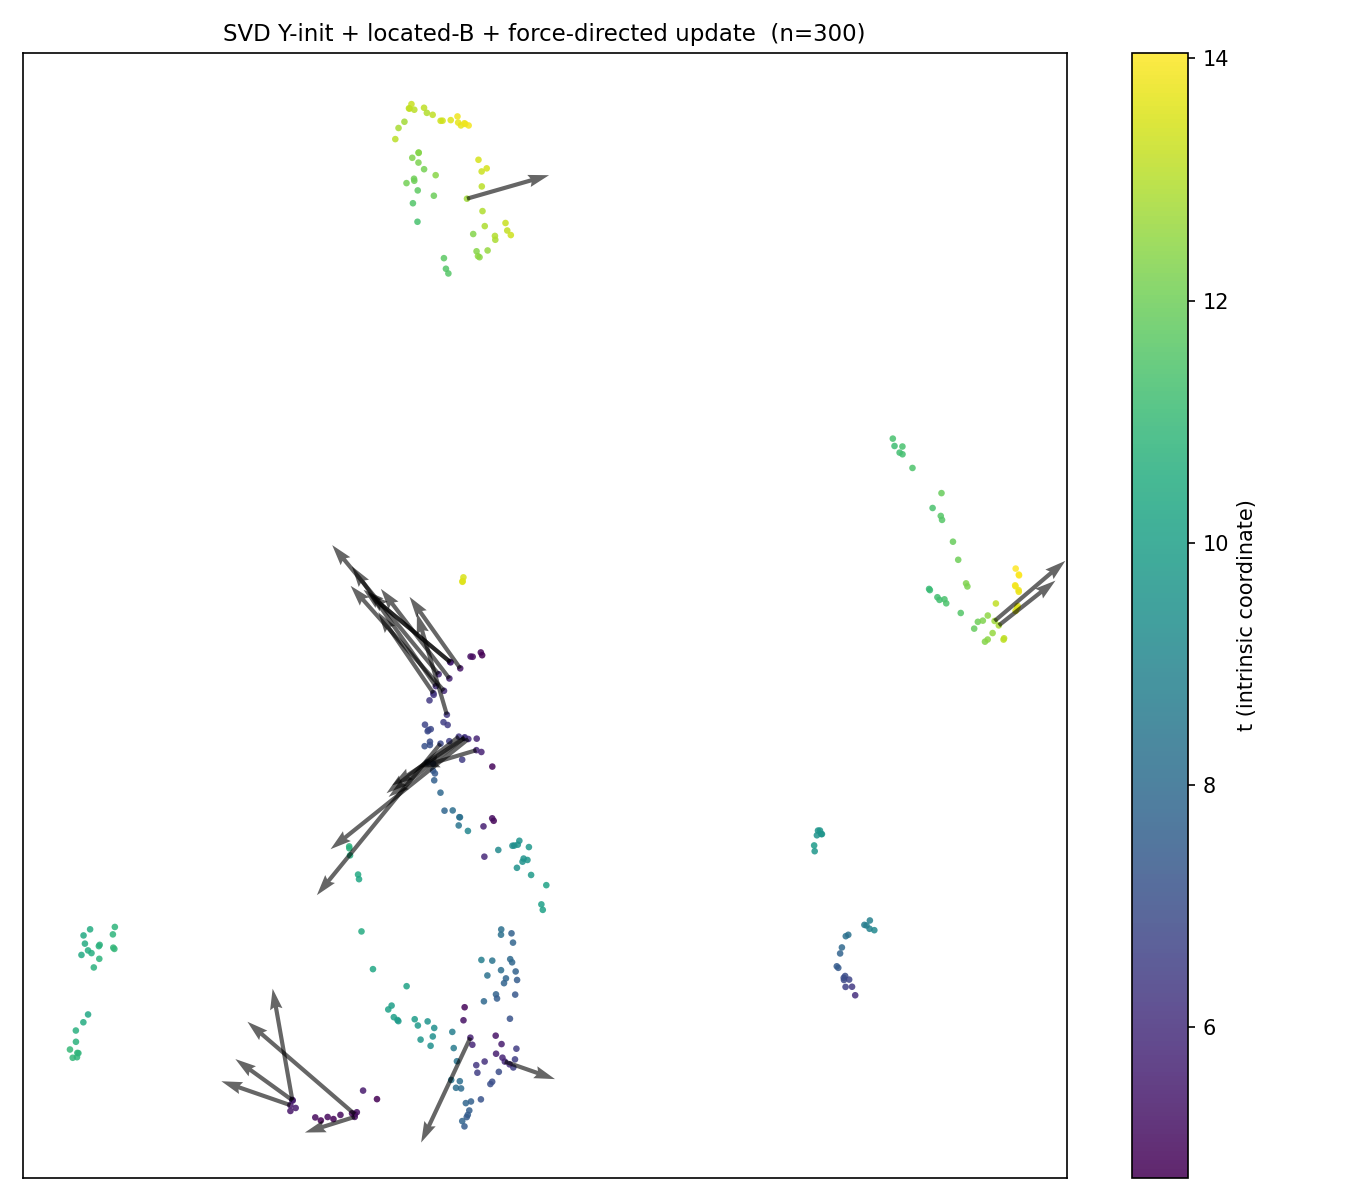
\includegraphics[width=\linewidth]{report_figs/final_svd.png}
\caption{SVD-RADAR $Y_{\mathrm{init}}$ + located $B$}
\end{subfigure}
\caption{$n=300$, 150 epochs, \texttt{ramp=False}, same seed/data across all three -- for direct
comparability rather than best-case tuning. All three still fragment into disconnected islands at
this epoch count; see \S\ref{sec:next}.}
\label{fig:three-methods}
\end{figure}

\section{This week's changes}
\label{sec:progress}

\begin{enumerate}
\item \textbf{Geodesic backbone rewritten to match lwileczek/isomap.} \texttt{compute\_dist\_matrix}
previously built its neighbourhood graph via scikit-learn's \texttt{kneighbors\_graph} (exactly $k$
neighbours per point, adaptive to local density). It now uses a single global distance threshold
$\varepsilon$ (\texttt{dist<}$\varepsilon$ $\Rightarrow$ edge), matching
\href{https://github.com/lwileczek/isomap}{lwileczek/isomap}'s \texttt{make\_adjacency} at the
advisor's request. $\varepsilon$ is auto-derived from $k$ so existing call sites are unaffected:
$\varepsilon(k)=\max_i d_k(i)$, the largest per-point $k$-th-nearest-neighbour distance in the
dataset.
\item \textbf{Diagnosed and fixed geodesic-backbone contamination.} Because $\varepsilon(k)$ is a
single \emph{global} value (set by the sparsest point), points in denser regions can end up
connected to ambient neighbours across different windings of the roll -- a classic Isomap
short-circuit. Measured directly: at $n=300$, $k=20$, the true geodesic 20-NN of some points reach
as far as $|t_i-t_j|=6.87$ (75\% of the entire $t$-range) -- structurally wrong. Reducing $k$
(20$\to$12) is provably safe against this specific failure mode, since $\varepsilon$ is monotone
non-decreasing in $k$: at $n=2000$, $k=12$, the same statistic drops to max $0.58$, median $0.11$ --
clean. (This is independent of the ramp finding in \S\ref{sec:ramp}, which turned out to hinge more
on locate-step convergence than on $k$ -- see the caveat there.)
\item \textbf{\texttt{snapshot\_every} added to both update mechanisms.} Both
\texttt{randers\_umap\_fit} and \texttt{finsler\_mds\_freeB} now record $(Y,B)$ every $N$ epochs
(epoch~0 = true pre-training init, final epoch always included even under early stopping), enabling
the trajectory grids used throughout this report and Figures~\ref{fig:ramp-off}--\ref{fig:ramp-on}.
\item \textbf{\texttt{ramp} exposed as a CLI flag everywhere.} \texttt{run\_swiss\_roll.py},
\texttt{run\_swiss\_roll\_isumap.py}, and \texttt{run\_swiss\_roll\_svd\_radar.py} all take
\texttt{--ramp} now (default off, matching the "locate once, freeze, attach at full strength"
design intent) -- previously \texttt{run\_swiss\_roll\_isumap.py} silently used
\texttt{randers\_umap\_fit}'s own \texttt{ramp=True} default without exposing it, an inconsistency
caught while reviewing the three scripts side by side.
\item \textbf{\texttt{run\_swiss\_roll\_svd\_radar.py} redesigned.} Previously: SVD init feeding
\texttt{finsler\_mds\_joint.py::finsler\_mds\_freeB}, an Adam optimiser minimising the Finsler
reconstruction loss $\sum(F(i\to j)-D_{\mathrm{asym}}[i,j])^2$ -- a fundamentally different
mechanism (gradient descent against a target matrix) from the other two scripts' force-directed
layout. Rewritten to use \texttt{randers\_umap\_fit} instead, per \S\ref{sec:three-methods}, so all
three scripts are now directly comparable on the same update rule.
\texttt{finsler\_mds\_joint.py} itself is untouched and still importable for anyone who wants the
Adam/loss variant.
\end{enumerate}

\section{Open items}
\label{sec:next}

\begin{enumerate}
\item \textbf{Isolate $k$ vs.\ locate-epochs in Table~\ref{tab:clip}.} Rerun $k=12$ with the full
500-epoch locate step (not 100) to separate the two confounded variables cleanly.
\item \textbf{Figure~\ref{fig:three-methods} still fragments at $n=300$, 150 epochs.} This is the
same dense-force-at-scale limitation flagged in the previous located-drift report
(\texttt{vanilla\_n300.png}, drift completely off, still fragments) -- not new, not fixed this
week. A longer run (300+ epochs, per the direction-accuracy plateau found earlier) and/or a genuine
stochastic-negative-sampling implementation (replacing the current dense all-pairs approximation)
remain the two live candidates.
\item \textbf{Direction-accuracy comparison across all three methods.} Every image in this report is
judged visually; a quantitative \texttt{direction\_accuracy\_swiss}-style comparison (recovered
$B$ vs.\ true $\omega$, projected into each embedding) across Isomap / isumap / SVD-RADAR has not
yet been run this week.
\item \textbf{Server-scale ($n\ge1000$) reruns of Figure~\ref{fig:three-methods}.} All three-way
comparisons here are at $n=300$ for turnaround speed; the $n=2000$ regime (where the ramp finding
actually matters) has only been tested for the Isomap script, not yet isumap or SVD-RADAR.
\end{enumerate}

\section*{Code}
\begin{center}
\begin{tabular}{@{}ll@{}}
\toprule
file & this week's role \\
\midrule
\texttt{randers\_bridge.py} & rewritten: eps-threshold backbone (item 1--2) \\
\texttt{randers\_umap.py} & \texttt{snapshot\_every}, \texttt{ramp} (already existed, now exposed) \\
\texttt{run\_swiss\_roll.py} & \texttt{--ramp}, \texttt{--snapshot-every} CLI flags added \\
\texttt{run\_swiss\_roll\_isumap.py} & \texttt{--ramp} CLI flag added (was silently on) \\
\texttt{run\_swiss\_roll\_svd\_radar.py} & rewritten: force-directed update, SVD $Y_{\mathrm{init}}$ + located $B$ \\
\texttt{finsler\_mds\_joint.py} & \texttt{snapshot\_every} semantics aligned; no longer wired into svd\_radar script \\
\bottomrule
\end{tabular}
\end{center}

\end{document}
